\section{System Architecture and Proposed Methodology}
The \textbf{X-IDS} framework is engineered to execute real-time, highly accurate, and fully interpretable intrusion detection strictly within the boundaries of Edge computing. This section details the structural design of the streaming pipeline, the hardware considerations of the Edge deployment, and the mathematical integration of Explainable AI (XAI).

\subsection{Real-Time Distributed Pipeline (Apache Kafka)}
A critical requirement for modern IDS is the ability to ingest and analyze network telemetry with zero downtime, even during massive volumetric attacks. Traditional Edge models often fail because processing bottlenecks cause localized memory buffer overflows, resulting in dropped packets. To resolve this, X-IDS integrates a distributed \textbf{Apache Kafka} architecture as the primary message broker.

Network flows, aggregated from external sensors or switch SPAN ports, are serialized into lightweight JSON payloads and published to localized Kafka topics. Kafka operates as a highly durable, fault-tolerant buffer. During traffic spikes (e.g., a Botnet DDoS attack), Kafka seamlessly queues the excess telemetry on disk, decoupling the high-velocity ingestion rate from the Edge device's finite inference speed. The localized machine learning engine subsequently consumes these micro-batches in a controlled, continuous stream, entirely eliminating hardware saturation and systemic packet loss.

\subsection{Edge Deployment: Raspberry Pi Hardware Optimization}
The core inference engine of X-IDS is deployed on a \textbf{Raspberry Pi 4 Model B}, equipped with a Broadcom BCM2711 localized Quad-core Cortex-A72 processor and rigidly capped at 4GB of RAM. Deploying deep neural networks or unoptimized ensemble models natively on this hardware is unfeasible; memory exhaustion occurs within minutes of active traffic ingestion.

To overcome these constraints, the X-IDS deployment strategy is twofold:
\begin{enumerate}
    \item \textbf{Algorithmic Selection:} We utilize LightGBM (Light Gradient-Boosting Machine) as the foundational inference model. LightGBM's Histogram-based decision tree algorithms and Exclusive Feature Bundling (EFB) allow it to process the massive throughput of network telemetry with an exceptionally low memory footprint compared to traditional XGBoost or deep learning arrays.
    \item \textbf{Micro-Batch Processing:} The inference engine consumes the Kafka stream via PySpark natively on the Pi. The execution environment is aggressively tuned—restricting the JVM memory allocation to 2GB and disabling non-essential Spark Web UIs—allocating exact resources to maintain a steady micro-batch processing latency of under 500ms.
\end{enumerate}

\subsection{XAI Integration via SHAP}
The foundational innovation of X-IDS is the operationalization of Explainable AI. We utilize \textbf{SHapley Additive exPlanations (SHAP)}, derived from cooperative game theory, not merely as an analytical luxury, but as a core architectural component.

SHAP calculates the precise marginal contribution of every variable to the model's final binary decision. Specifically, for an IDS model $f(x)$ and a network flow $x$, the SHAP value $\phi_i$ for an individual feature $i$ is calculated by evaluating the outcome across all possible combinations of features $S$:
\begin{equation}
    \phi_i(f, x) = \sum_{S \subseteq N \setminus \{i\}} \frac{|S|! (M - |S| - 1)!}{M!} \left( f_x(S \cup \{i\}) - f_x(S) \right)
\end{equation}
where $M$ is the total domain of features, and $f_x(S)$ is the prediction expected given the subset $S$.

\subsubsection{Global Interpretability for Edge Pruning}
Pre-deployment, we leverage Global SHAP values—the mean absolute magnitude of $\phi_i$ across the entire CICIDS2017 training matrix—to conduct aggressive dimensionality reduction. We prove mathematically that $>60\%$ of the standard 78 network features (e.g., isolated ACK flags, minor variance measurements) contribute statistically zero weight to the classification boundary. By mathematically pruning the input vector to the Top-30 most impactful features, X-IDS directly reduces the RAM required for the Spark \texttt{VectorAssembler} by over $40\%$, allowing the model to fit flawlessly on the Raspberry Pi.

\begin{figure}[htbp]
\centering
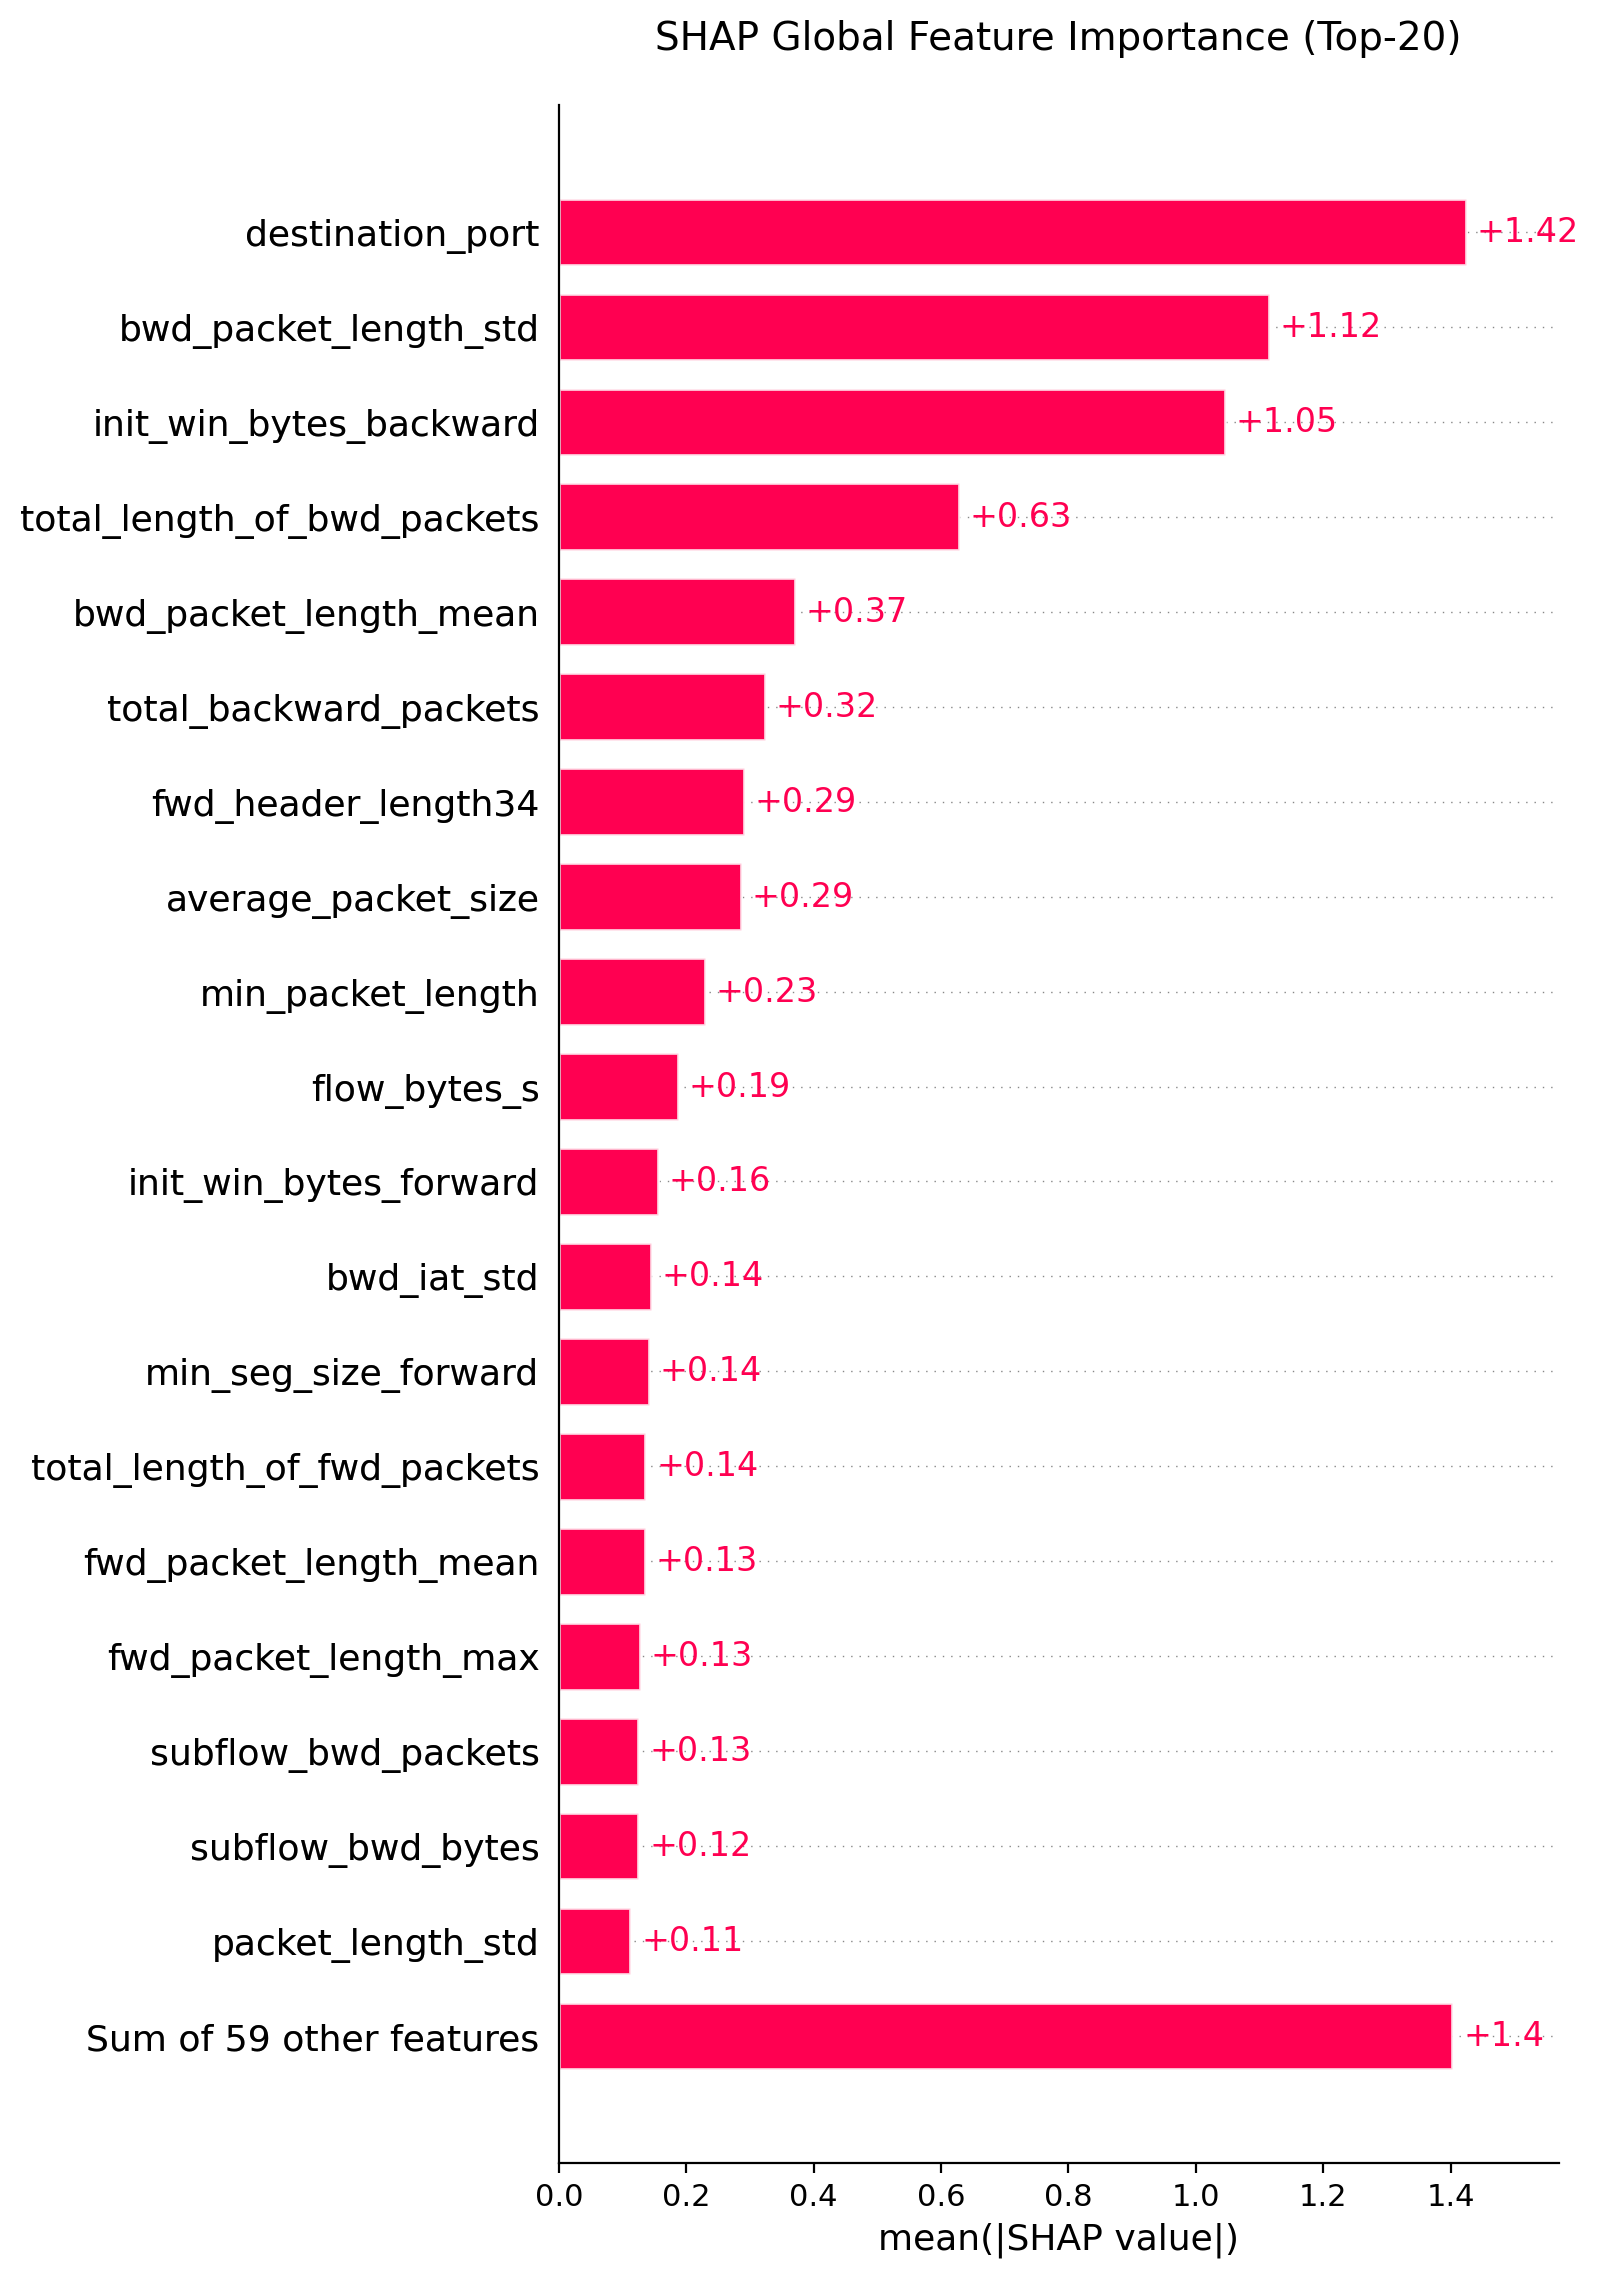
\includegraphics[width=\columnwidth]{figures/shap_feature_importance_bar.png}
\caption{Global SHAP Feature Importance, indicating that only a subset of network features provide meaningful predictive weight.}
\label{fig:shap_bar}
\end{figure}
\subsubsection{Local Interpretability for Real-Time Trust}
Post-deployment, X-IDS generates Local SHAP explanations for every triggered alert in real-time. Instead of presenting a SOC analyst with an opaque "Malicious" flag, the system dynamically outputs an exact mathematical attribution. For example, if a \textit{Slowloris} attack triggers an alert, the SHAP engine immediately highlights \texttt{Flow Duration} and \texttt{Bwd Packet Length Min} as the primary causal vectors driving the decision. This localized, human-readable transparency definitively cracks the black-box, empowering incident responders with the actionable, trusted intelligence required to immediately isolate compromised network nodes.

\begin{figure}[htbp]
\centering
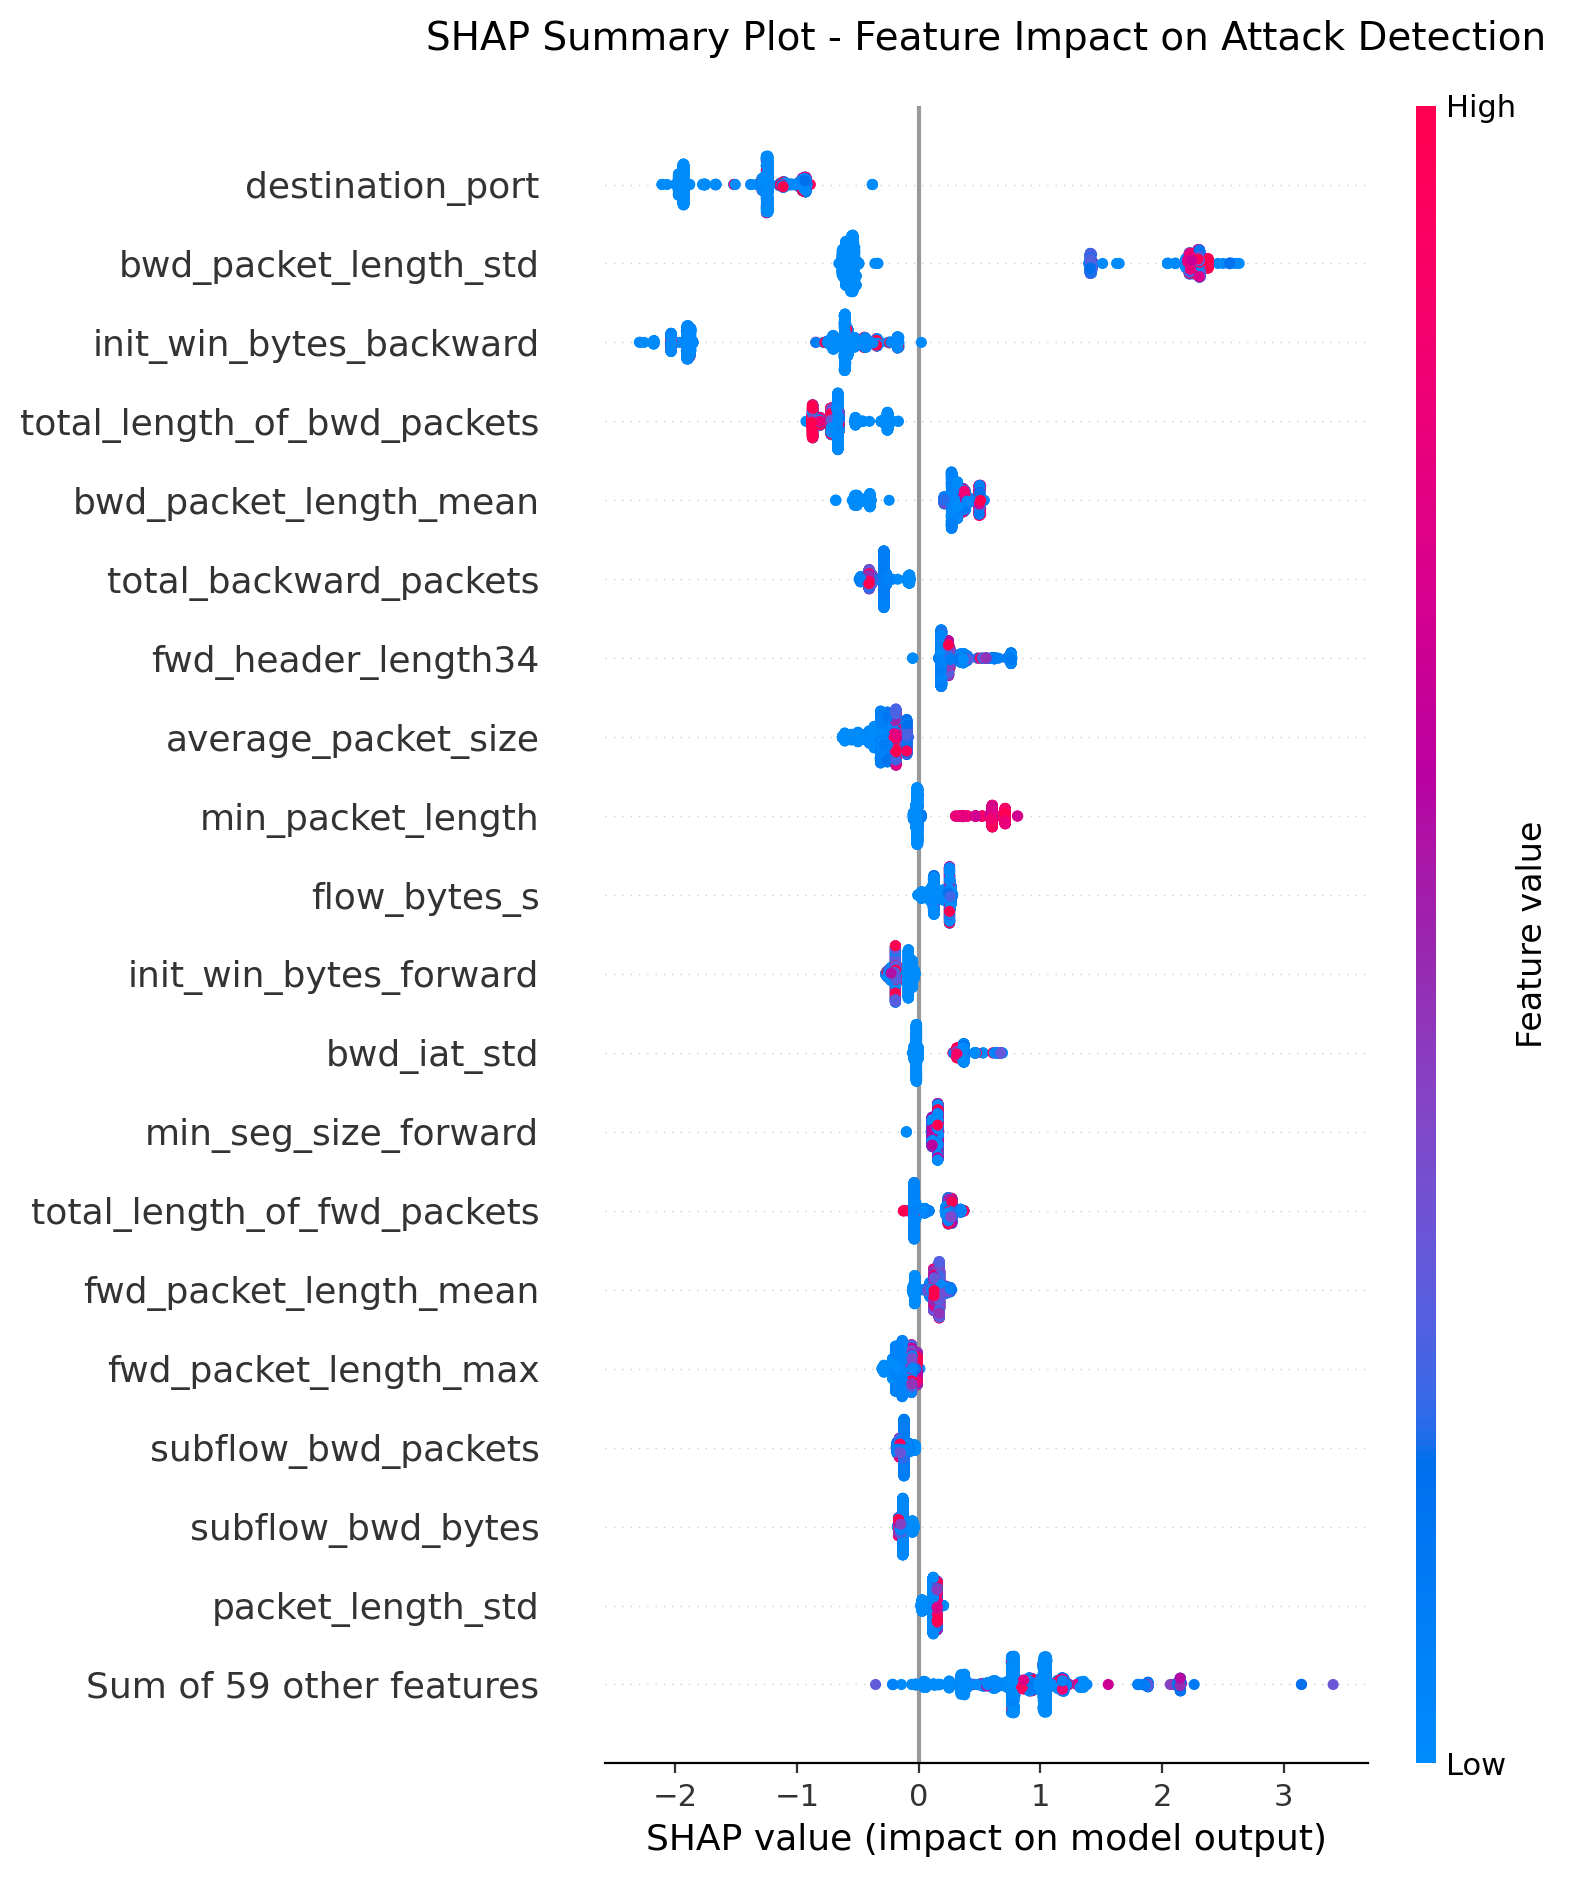
\includegraphics[width=\columnwidth]{figures/shap_summary_beeswarm.png}
\caption{SHAP Summary Beeswarm plot detailing the distribution of feature impacts on model output across multiple attack vectors.}
\label{fig:shap_beeswarm}
\end{figure}
